% Copyright (c) 2026 CorrectBrain
% SPDX-License-Identifier: MIT

\PassOptionsToPackage{dvipsnames,svgnames,x11names}{xcolor}
\documentclass[tikz,border=8pt]{standalone}
\usetikzlibrary{arrows.meta,positioning,calc,shapes,shadows,decorations.pathmorphing,shapes.geometric,backgrounds,decorations.markings,decorations.pathreplacing,decorations.text,fit,shapes.misc,shapes.arrows,matrix,bending,3d,chains,intersections,shapes.symbols,svg.path,shapes.multipart,snakes,shapes.callouts,angles,quotes}
\providecolor{gold}{RGB}{212,175,55}
\providecolor{silver}{RGB}{192,192,192}
\providecolor{bronze}{RGB}{205,127,50}
\providecolor{darkblue}{RGB}{0,0,139}
\providecolor{lightblue}{RGB}{173,216,230}
\providecolor{darkgreen}{RGB}{0,100,0}
\providecolor{lightgreen}{RGB}{144,238,144}
\providecolor{darkred}{RGB}{139,0,0}
\providecolor{navy}{RGB}{0,0,128}
\providecolor{skyblue}{RGB}{135,206,235}
\providecolor{beige}{RGB}{245,245,220}
\providecolor{cream}{RGB}{255,253,208}
\usepackage{amsmath}
\usepackage{amssymb}
\usepackage{fontawesome5}
\usetikzlibrary{fadings,shadows.blur,patterns,patterns.meta}

\usepackage[T1]{fontenc}
\usepackage{lmodern}
\usepackage{tikz}
\usepackage{xcolor}

\definecolor{timegray}{RGB}{149, 165, 166}
\definecolor{mainthread}{RGB}{231, 76, 60}
\definecolor{preparser}{RGB}{46, 204, 113}
\definecolor{network}{RGB}{52, 152, 219}
\definecolor{darkgray}{RGB}{44, 62, 80}
\definecolor{goodgreen}{RGB}{39, 174, 96}

\begin{document}
\begin{tikzpicture}[
    box/.style={
        draw=black!15,
        fill=white,
        rounded corners=4pt,
        drop shadow={opacity=0.15, shadow xshift=1pt, shadow yshift=-2pt},
        align=center,
        inner sep=8pt,
        font=\sffamily\small,
        text=darkgray
    },
    timeline/.style={very thick, dashed, timegray},
    event/.style={circle, fill=white, draw=timegray, thick, inner sep=2pt, font=\tiny\sffamily\bfseries, text=darkgray},
    arrow/.style={-Stealth, thick, darkgray}
]

% ==========================================
% TITLE SECTION (y = 12)
% ==========================================
\node[font=\Huge\bfseries\color{darkgray}] at (14, 12.4) {The Web Performance Race};
\node[font=\Large\color{darkgray!80}] at (14, 11.6) {Why layout constraints are resolved \textit{before} the main CSS thread resumes};

% ==========================================
% COLUMNS HEADER (y = 10.5)
% ==========================================
\node[font=\large\bfseries\color{timegray}] at (0, 10.5) {Time};
\node[font=\large\bfseries\color{mainthread}] at (6, 10.5) {\faCogs \ Main Thread (Parser)};
\node[font=\large\bfseries\color{preparser}] at (14, 10.5) {\faSearch \ Pre-load Scanner};
\node[font=\large\bfseries\color{network}] at (22, 10.5) {\faWifi \ Network / Layout};

% Timeline vertical dashed lines on lower background layer with global solid white canvas
\begin{scope}[on background layer]
    \fill[white] (-2, -10) rectangle (28, 14);
    \draw[timeline] (0, 10.0) -- (0, -9.2);
    \draw[timeline] (6, 10.0) -- (6, -9.2);
    \draw[timeline] (14, 10.0) -- (14, -9.2);
    \draw[timeline] (22, 10.0) -- (22, -9.2);
\end{scope}

% Dedicated Isolated Network Download Stream (x = 26.0, spans strictly from y = 4 to y = -8)
\fill[top color=network!50, bottom color=network!15, draw=network!70, thick, rounded corners=3pt] (25.7, -8) rectangle (26.3, 4);
\node[rotate=90, font=\scriptsize\sffamily\bfseries, text=network!90!black, fill=white, inner sep=2pt, rounded corners=2pt] at (26.0, -2) {\faDownload\ Downloading Image Data};

% ==========================================
% WATERFALL EVENTS
% ==========================================

% --- t = 0ms (y = 8) ---
\node[event] at (0, 8) {0ms};
\node[box, draw=mainthread, line width=1.2pt, text width=5.0cm] (main0) at (6, 8) {
    {\color{mainthread}\textbf{\normalsize Start Parsing}}\\[2pt]
    {\footnotesize Read HTML top-down}
};
\node[box, draw=network, line width=1.2pt, text width=5.0cm] (net0) at (22, 8) {
    {\color{network}\textbf{\normalsize HTML Payload Arrives}}\\[2pt]
    {\footnotesize First bytes stream in}
};
\draw[arrow, network] (net0.west) -- (main0.east) node[midway, above=3pt, font=\scriptsize\sffamily\bfseries, text=darkgray, fill=white, inner sep=2pt] {Network Buffer};

% --- t = 5ms (y = 4) ---
\node[event] at (0, 4) {5ms};
\node[box, draw=mainthread, line width=1.2pt, text width=5.0cm] (main5) at (6, 4) {
    {\color{mainthread}\textbf{\normalsize Blocked by CSS/JS}}\\[2pt]
    {\footnotesize Main parser encounters \texttt{<link>} or \texttt{<script>} and pauses.}
};
\node[box, draw=preparser, line width=1.2pt, text width=5.0cm, fill=preparser!6] (scan5) at (14, 4) {
    {\color{preparser!90!black}\textbf{\normalsize Scanner Races Ahead!}}\\[2pt]
    {\footnotesize Finds \texttt{<img width="800" height="400">}.\\Computes Aspect Ratio = \textbf{2:1}}
};
\draw[arrow, preparser] (main5.east) -- (scan5.west) node[midway, above=3pt, font=\scriptsize\sffamily\bfseries, text=preparser!90!black, fill=white, inner sep=2pt] {Spawns};
\draw[arrow, network] (scan5.east) -- (25.7, 4) node[midway, above=3pt, font=\scriptsize\sffamily\bfseries, text=network!90!black, fill=white, inner sep=2pt] {Initiate Image Request};

% --- t = 15ms (y = 0) ---
\node[event] at (0, 0) {15ms};
\node[box, draw=preparser, line width=1.2pt, text width=5.0cm] (scan15) at (14, 0) {
    {\color{preparser!90!black}\textbf{\normalsize Speculative Space Request}}\\[2pt]
    {\footnotesize Sends 2:1 ratio data to layout engine prematurely.}
};
\node[box, draw=network, line width=1.2pt, text width=5.0cm, fill=network!6] (layout15) at (22, 0) {
    {\color{network}\textbf{\normalsize Layout Engine}}\\[2pt]
    {\footnotesize Allocates empty placeholder box (800x400) in DOM memory.}\\[3pt]
    \tikz[baseline=-0.5ex]{\draw[thick, dashed, network, fill=network!15, rounded corners=2pt] (0,0) rectangle (2.2, 1.1) node[midway, font=\scriptsize\sffamily\bfseries, text=network!90!black] {2:1 (800$\times$400)};}
};
\draw[arrow, preparser] (scan15.east) -- (layout15.west);

% --- t = 50ms (y = -4) ---
\node[event] at (0, -4) {50ms};
\node[box, draw=mainthread, line width=1.2pt, text width=5.0cm] (main50) at (6, -4) {
    {\color{mainthread}\textbf{\normalsize CSS Executed}}\\[2pt]
    {\footnotesize Main thread resumes. Applies \texttt{max-width: 100\%;}.\\Uses pre-calculated 2:1 ratio for fluid \texttt{height}.}
};

% Orthogonal Feedback arrow from Layout Engine to Main Thread (CSS Execution) strictly progressing forward through time
\draw[arrow, darkgray, dashed, rounded corners=6pt]
    (layout15.south) -- (22, -2) -- (6, -2)
    node[midway, above=2pt, font=\scriptsize\sffamily\bfseries, text=darkgray, fill=white, inner sep=2pt] {Layout constraints fed back}
    -- (main50.north);

% --- t = 200ms (y = -8) ---
\node[event] at (0, -8) {200ms};
\node[box, draw=goodgreen, line width=1.2pt, text width=5.0cm, fill=goodgreen!8] (net200) at (22, -8) {
    {\color{goodgreen!90!black}\textbf{\normalsize Image Bytes Finish}}\\[2pt]
    {\footnotesize Pixels stream into the \textbf{already perfectly sized} placeholder box.}\\[3pt]
    {\bfseries\color{goodgreen!80!black}\faCheckCircle\ Zero Layout Shift!}
};

% Download Data Flow Arrow into finished image node
\draw[arrow, network] (25.7, -8) -- (net200.east);

\end{tikzpicture}
\end{document}
